\chapter{Kiểm thử hệ thống}
\subsection{Tổng quan về kiểm thử}

Mục đích của kiểm thử trong hệ thống: Đảm bảo rằng các tính năng hoạt động đúng, hệ thống không có lỗi và có thể chịu được tải trong quá trình sử dụng thực tế.

Loại kiểm thử thực hiện:
\begin{itemize}
	\item \textbf{Kiểm thử chức năng:} Đảm bảo các chức năng của hệ thống hoạt động đúng
	\item \textbf{Kiểm thử hiệu suất:} Đảm bảo hệ thống có thể xử lý nhiều yêu cầu đồng thời
	\item \textbf{Kiểm thử bảo mật:} Đảm bảo hệ thống bảo vệ tốt các dữ liệu người dùng
	\item \textbf{Kiểm thử tích hợp:} Kiểm tra sự hoạt động đồng bộ của các module
	\item \textbf{Kiểm thử hồi quy:} Đảm bảo những thay đổi mới không làm hỏng các tính năng cũ
\end{itemize}


\subsection{Mô tả chung về các kịch bản kiểm thử}

Mỗi kịch bản kiểm thử được tổ chức và theo dõi theo bảng sau đây. Các mục chính trong mỗi kịch bản kiểm thử bao gồm:
\begin{itemize}
	\item \textbf{TEST SCENARIO:} Tên kịch bản kiểm thử
	\item \textbf{Screen name/Function name:} Tên màn hình hoặc tên chức năng cần kiểm thử
	\item \textbf{Test case code:} Mã số của test case
	\item \textbf{Number of passed test cases (P):} Số lượng test case đã thành công
	\item \textbf{Number of failed test cases (F):} Số lượng test case không thành công
	\item \textbf{Number of test cases under pending (PE):} Số lượng test case đang chờ xử lý
	\item \textbf{Number of unexecuted test cases:} Số lượng test case chưa được thực hiện
	\item \textbf{Total number of test cases:} Tổng số test case cần kiểm thử
\end{itemize}

\subsubsection{Cấu trúc của một kịch bản kiểm thử}

\begin{itemize}
	\item \textbf{Test case code:} Mã của test case, giúp phân biệt các test case khác nhau
	\item \textbf{Testing Purpose:} Mục đích của việc kiểm thử
	\item \textbf{Steps:} Các bước thực hiện kiểm thử
	\item \textbf{Expected outcome:} Kết quả mong đợi sau khi thực hiện các bước kiểm thử
	\item \textbf{Browser compatibility testing:} Kiểm tra tính tương thích với các trình duyệt phổ biến
	\item \textbf{Test status report:} Báo cáo tình trạng của các lần kiểm thử
\end{itemize}

\subsubsection{Ví dụ về một kịch bản kiểm thử trong bảng Excel}
\begin{figure}[H]
	\centering
	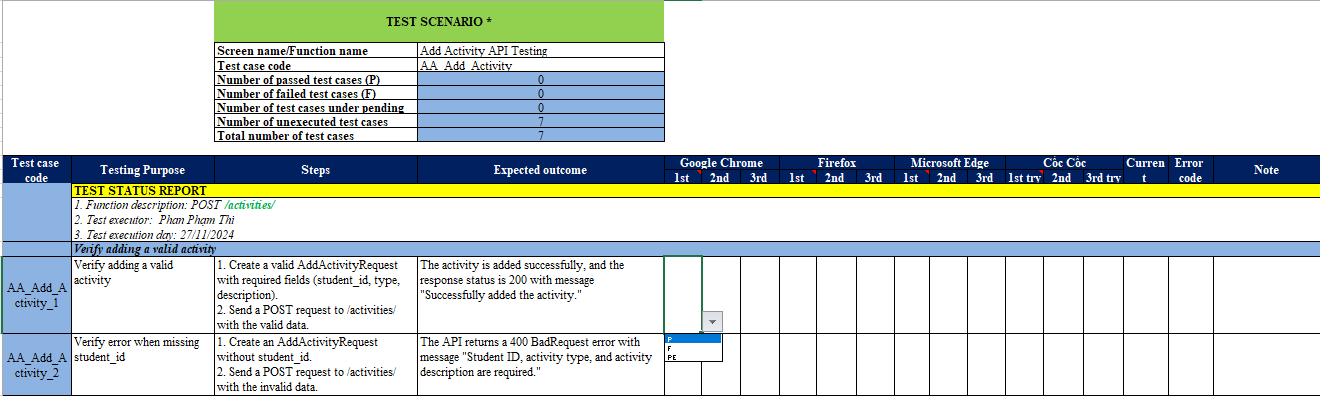
\includegraphics[scale=0.5]{Images/Implement/testScenario.png}
	\caption{Ví dụ về một kịch bản kiểm thử}
\end{figure}
\subsubsection{Mục tiêu của các kịch bản kiểm thử}
\begin{itemize}
	\item \textbf{Kiểm thử chức năng}: Đảm bảo các API hoạt động đúng với các yêu cầu và dữ liệu đầu vào hợp lệ hoặc không hợp lệ.
	\item \textbf{Kiểm thử tương thích trình duyệt}: Đảm bảo hệ thống hoạt động ổn định trên các trình duyệt phổ biến.
	\item \textbf{Kiểm thử độ tin cậy}: Kiểm tra xem các API có thể xử lý được các tình huống thực tế và đưa ra kết quả chính xác.
\end{itemize}

\section{Các API cần kiểm thử}
Các APIs được kiểm thử sẽ là các APIs có liên quan đến các chức năng chính của hệ thống như:
\begin{itemize}
	\item Sinh ra lộ trình học tập cho sinh viên
	\item Gợi ý mục tiêu học tập cho sinh viên đối với một khóa học cụ thể
	\item Sinh ra bài tập quiz tự động cho sinh viên
	\item Đánh giá kết quả học tập của sinh viên
	\item Tái tạo nội dung bài học cho sinh viên
\end{itemize}

\section{Kết quả kiểm thử API}
\subsection{Kết quả tổng hợp của các testcase}
\begin{figure}[H]
	\centering
	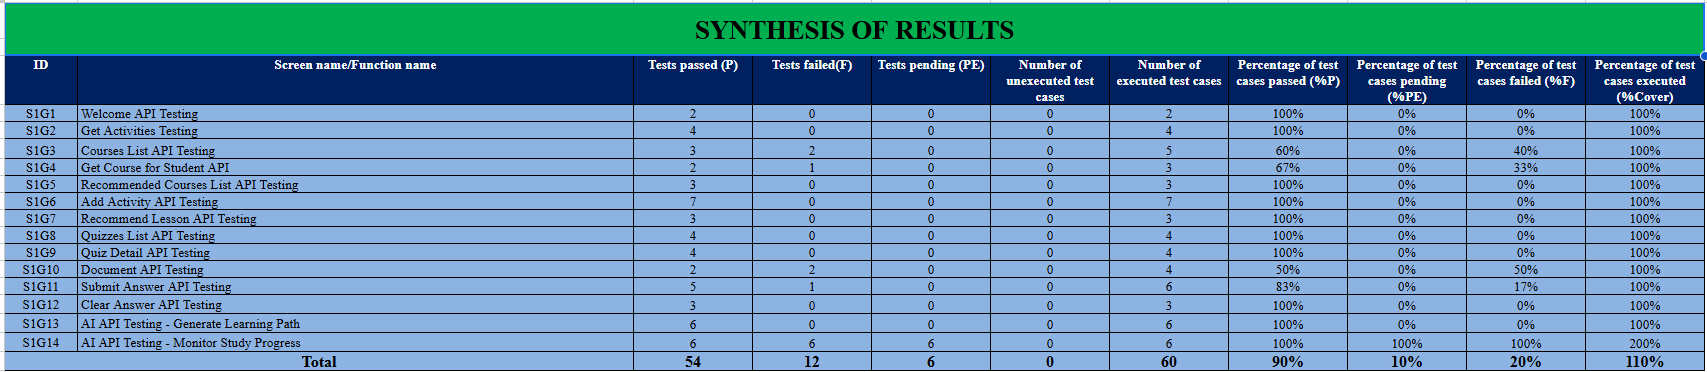
\includegraphics[width=0.8\textwidth]{Images/test/synthesisResults.png}
	\caption{Kết quả tổng hợp của các testcase}
\end{figure}
\begin{itemize}
	\item \textbf{Số lượng test case đã thực thi:} Toàn bộ 60 test case đã được thực thi, đạt tỷ lệ bao phủ kiểm thử là 100\%.
	\item \textbf{Số lượng test case đã vượt qua:} Có 54 test case thành công, chiếm 90\% tổng số test case.
	\item \textbf{Số lượng test case thất bại:} Có 6 test case thất bại, chiếm 12\% tổng số test case.
	\item \textbf{Số lượng test case đang chờ xử lý:} Có 10 testcases đang chờ xử lý.
\end{itemize}

\section{Hạn chế}
\begin{itemize}
	\item Do nhóm chưa có nhiều kinh nghiệm trong việc thực hiện unit testing.
	\item Quá trình kiểm thử chủ yếu tập trung vào kiểm tra chức năng các API quan trọng mà chưa thực hiện đầy đủ các kiểm thử liên quan đến giao diện người dùng (UI testing) hoặc hiệu năng hệ thống (performance testing).
	\item Vẫn tồn tại một số lỗi cần được kiểm tra và sửa lỗi.
\end{itemize}
